%etig-term-paper.tex 
\documentclass[12pt]{article}
\usepackage{times}
\usepackage{amsmath,amssymb,latexsym}
\usepackage[round,sort]{natbib}
\usepackage{multirow,array}
\usepackage{fancyhdr}
\usepackage{lastpage}
\usepackage{graphicx}
\usepackage[bottom]{footmisc}
\graphicspath{ {etig-term-paper-presentation-images/} }
\usepackage[T1]{fontenc}
\usepackage{mathptmx}
\usepackage{tabu}
\usepackage{textcomp}
\usepackage{stata}
\usepackage{listings}
\usepackage[a4paper,margin=1.0in]{geometry}
\usepackage{multirow}
\usepackage{caption}
\usepackage{setspace}
\usepackage{verbatim}
\usepackage{pdflscape}
\usepackage{longtable}
\usepackage{hyperref}
\setlength{\parindent}{4pt}
\setlength{\parskip}{1.2em}
\hypersetup{
    colorlinks=true,
    linkcolor=blue,
    filecolor=magenta,      
    urlcolor=cyan,
    citecolor=magenta,
}
\lstset{
basicstyle=\ttfamily,
columns=flexible,
breaklines=true
}
\newenvironment{hypothesis}{
  	\itshape
  	\leftskip=\parindent \rightskip=\parindent
  	\noindent\ignorespaces}
	
\setlength\parindent{0pt}
\pagestyle{fancy}
\fancyhf{}

\lhead{Does inventor mobility affect complexity of inventors\textquotesingle \ inventions?}

\rfoot{Page \thepage  \ of \pageref{LastPage}}
\rhead{Iyenggar}
\newcommand\question[2]{\vspace{1em}\hrule\vspace{1em}\textbf{#1}{ #2}\vspace{1em}\hrule\vspace{1em}}

\begin{document}

\title{\LARGE Does inventor mobility affect complexity of inventors\textquotesingle \ inventions?\\ \Large \textit{Economics of Technology, Innovation and Growth} \\course term paper}

\author{Ashwin Iyenggar  (1521001) \\ ashwin.iyenggar15@iimb.ernet.in} 
\large

\maketitle
\thispagestyle{empty}

\begin{abstract}
\large \noindent Using patent inventions data, I attempt to investigate if inventor mobility influences the complexity of inventions made by inventors. I leverage a database of worldwide urban regions  obtained from remote sensing to demonstrate a significant positive correlation between both inter-region mobility  and inter-country mobility and future complexity of inventions of inventors. I discuss two additional approaches to investigate if a causal explanation exists for this relationship but leave empirical analysis for future work. While the empirical results are incomplete, the current work extends prior work on mobility of inventors by attempting to quantify the direct effects of  mobility on complexity of inventions.
\end{abstract}
{Keywords:} complexity of inventions, Inventor mobility, Economic geography
\onehalfspacing
\section{Introduction}
Scholars have suggested that inventors carry knowledge with them when they move \citep{Almeida1999}. While the literature on knowledge flows has investigated the localized nature of knowledge flow driven by the inter-firm mobility of inventors \citep{Jaffe1993, Almeida1999, Alcacer2006a}, we understand very little about the effects of broad mobility of inventors on future inventive complexity. Since firms, regions and countries seek to organize themselves so as to attract the best inventors so as to produce the highest level of innovative output, an understanding of the mobility effects of inventive complexity becomes an important aspect innovation policy. In this paper I ask if  the variation in inventor mobility can explain the variation in invention complexity?

Agglomeration economies have been suggested as one reason for localized movement of inventors. These agglomeration economies arise due to labor pooling advantages, economies of specialization of local suppliers, and knowledge spillovers \citep{Porter1990, Krugman1991}. However regions vary in their inventive output \citep{Agrawal2014} and the nature of knowledge flows in a region may be one source of this variation within regions. In this study therefore, I propose to expand the context to not just localized agglomerations but to all movements of inventors. By doing so, I expect to understand if there is a clear impact of mobility itself on invention complexity. In other words, what is the relationship between the movement of some inventors into or out of a region and the average complexity of inventions from those inventors?\par

There has been a long and illustrious scholarly tradition highlighting the agglomeration characteristics of economic regions, going back at least as far as \cite{Marshall1890}, whose original work was published in 1890. More recently, scholars over the last three decades have demonstrated the paper trail of these knowledge spillovers through the study of patent citations (e.g., \cite{Jaffe1993, Almeida1999}). This tradition of scholarship has further shaped our theoretical understanding of knowledge spillovers through mechanisms such as the effects of inventor mobility (e.g., \cite{Almeida1999}), differential Intellectual Property Rights environments across locations (e.g., \cite{Zhao2006}) and of the role of international geography (e.g., \cite{Singh2007}).  The nature and extent of the geographical mobility of inventors  observed  in practice is highly heterogenous across locations, firms and legal environments. This raises the opportunity to study if  a causal effect exists between mobility of inventors and their future complexity. The question is assumes greater significance in the environment surrounding the second machine age \citep{Mcafee2014} where inventors are expected to influence innovation outcomes in higher proportion. 

The innovation policy of emerging countries is influenced with the expectation that the presence of multinational R\&D will create value adding spillover effects. complexity of inventors may  provide a richer proxy for value adding innovation. A better understanding of the effects of inventor mobility may therefore help to inform innovation policy. Additionally, work on this line may help to inform managerial decisions about how to organize R\&D teams around the world. Current theory seems to suggest both a positive effect due to knowledge spillovers \citep{Almeida1999} as well as a negative effect due to variation in IPR enforcement ability \citep{Zhao2006}. I therefore propose  the current empirical study to help determine an  answer to this question that is not completely explained by theory.

The rest of the paper is organized as follows. The next section explores the motivation of the current study through a preliminary analysis of the data. Hypotheses based on extant literature are then presented. I then describe the data and methods. The preliminary results are then presented, followed by a discussion of the results. I conclude with next steps and open questions for further research.


\section{Preliminary Analysis}
I motivate this study by demonstrating two broad patterns.  First, as Figure ~\ref{fig:countrymoves} suggests,  there has been increased mobility of inventors across countries over the years. Not only is the incidence of across-country mobility higher, but there is heterogeneity in the extent across countries and regions. Figure ~\ref{fig:regionmoves} furthers this aspect by depicting the trend in across-region mobility of inventors. Second, Table ~\ref{sumstat} suggests that about 8\% of inventors moved  and only about 3\% of inventors moved country. 

The two broad patterns together provide us both the motivation as well as the variation in the data to be able ask the question of whether the mobility of inventors affects invention complexity. It must be noted at this point that while we have data on inventors who moved and patented in their new location, and data on inventors who did not move and continued to patent at their existing location, the patents data itself does not provide us data on those inventors who moved but did not patent, and those who did not move and did not patent. This may cause us to either overestimate the effect of mobility or underestimate the effect of not moving. 

\section{Inventor Mobility and its Consequences}
In this section, I develop three hypothesis building off of prior literature on inventor mobility and knowledge spillovers. 

The literature on agglomeration economies and knowledge spillovers suggest that when inventors move across regions, that newer combinations of knowledge now become possible \cite{Jaffe1993, Almeida1999}. Literature would therefore predict better and more numerous inventions arising out of the movement of inventors. I therefore propose hypothesis 1 as follows:\par
\begin{hypothesis}{\\Hypothesis 1: An increase in the average mobility of inventors in a region increases the average complexity of  innovation generated}\end{hypothesis}

\cite{Singh2007} suggests that inventors who were highly productive previously are likely to carry that after the move. I therefore propose hypothesis 2 as follows:\par
\begin{hypothesis}{\\Hypothesis 2: The effect in Hypothesis 1 is moderated positively by the relative strength of the intellectual property rights regime of the region}\end{hypothesis}

Finally, the literature of weak and strong IPR suggests that teams within weak IPR locations are likely to integrate their knowledge within global organizations, thus leading to a lower standalone inventive output. I therefore propose hypothesis 3 as follows:\par
\begin{hypothesis}{\\Hypothesis 3: The effect in Hypothesis 1 is moderated negatively by the strength of the prior pool of inventions by the inventing team}\end{hypothesis}


\section{Method}
\subsection{Complexity}
Prior literature has suggested that complexity may be viewed as recombination of existing knowledge elements \citep{Fleming2001}. Additionally there is an extensive body of literature that suggests that technological innovation as a search on technology landscapes \citep{Kauffman1993, Levinthal1997}. In this article, I build on top of this notion of complexity as a recombination to define a measure of complexity of inventor inventions.

Since patents vary even within technology subclasses, I suggest an additional measure of complexity to capture additional variation in the data. I construct my measure of complexity based interactions between the different patent sub-classes. Since each of the interactions between patent sub-classes may introduce a new interaction, I model interactions on a binomial function. Specifically, when \verb|subclass| represents the number of distinct patent sub-classes, I define  \verb|interaction(subclass)| as follows:

\begin{displaymath}
   interaction(subclass) = \left\{
     \begin{array}{lr}
       1 & : subclass \leq 2 \\
       \binom{subclass}{2} & : subclass > 2 \\
     \end{array}
   \right.
\end{displaymath} 

I would expect, from a user perspective that the more number of contexts in which the patent is valuable, the lower should be the complexity. If \verb|complexity| represents my measure of the complexity of the patent, and \verb|usage contexts| represents the number of distinct contexts where the patent is found valuable, I should expect the following relationship to hold:
\begin{center}$ \verb|Complexity| \propto \frac{1}{usage \ contexts} $ \end{center}
Similarly, from an inventor perspective, the more the number of contexts that the patent is built on, the higher should be the complexity. A patent that is developed without citing any other patents is an extreme case of lowest complexity, while one that requires to be built upon several \verb|source contexts| is properly understood as being more complex. 

The relationship between \verb|source contexts| and \verb|complexity| is therefore a normal one as depicted below.
\begin{center}$ \verb|complexity| \propto source \ contexts $ \end{center} 

Using the principles above, I therefore develop the following definition of complexity.
\begin{center}$ \verb|complexity| = \frac{interaction(subclass_{\text{cited}})}{interaction(subclass_{\text{patent}})} $ \end{center}

By the definition above, a patent that cites no patents (and hence has $subclass_{\text{cited}} = 0$) but is itself assigned to 4 sub-classes (and hence has $subclass_{\text{patent}} = 4$) will have a raw Complexity score of $\frac{1}{\binom{4}{2}} = 0.16$. If the patent itself had been assigned onto to 2 sub-classes, the raw complexity score would have been just 1. Therefore, the more the number of patent sub-classes a patent is assigned to, the lower its complexity score (by a square term). A similar but inverse relationship would hold for sub-classes arising out of cited patents. Here, I take a set union of patent sub-classes assigned to each cited patent, and use that count to determine the value of the \verb|interaction| function.

\subsection{IPR Classification}
\cite{Zhao2006} has argued  that multinational enterprises may benefit from conducting R\&D in countries with weak IPR protection by  making up for the weaker IPR protection through better internal organization. An alternative specification may therefore be to include IPR score to capture shifts in the data. Scholars \citep{Yayavaram2008, Baldwin2015}, have argued that increased interaction with a larger number of components creates organizational impediments to an increase in reusability of prior work. In the presence of a stronger differential in the IPR environments between inventing locations, \cite{Zhao2006} suggests that organizational mechanisms may stand to counter the treat posed by weaker property rights. In a similar vein, I argue that a differential in the IPR rights environment creates the organizational response to increase complexity of the inventions shared across country and IPR boundaries. This may help capture an exogenous variation that may help identify the mobility-complexity relationship.

A review of the academic literature surrounding the construction of IPR indexes indicated that there were several, as was also evident in \cite{Zhao2006} constructing a composite measure for the purposes of her article. \cite{Lesser2010} provides an alternative, composite scoring system that includes the following components: protectable subject matter, membership in convention, enforcement, administration and duration of protection. I have therefore used the scores generated by \cite{Lesser2010} for the purposes of this study. The extensive table of IPR scores has not been presented here, but can be made available on request. The listing has several countries for which scores have not been provided. However none of the top patenting nations were among them, and I therefore chose to go along with this scale.

\section{Data and Measures}

I derive all patents data for this study from patentsview.org. The dataset considered is for all USPTO patents filed in the period 1976 to 2015. For country definitions, I use the resources provided by \href{http://thematicmapping.org/downloads/world_borders.php}{Thematic Mapping}. To map location data of inventors to regions, I use urban centers data for worldwide locations from \href{http://www.naturalearthdata.com/downloads/10m-cultural-vectors/}{Natural Earth Data} that uses remote sensing data to determine urban agglomerations (a process developed in \cite{Schneider2003}).  While it has been common practice to use Metropolitan Statistical Areas (MSA) for analyses related to economic geography in the U.S., an equivalent measure is unavailable for the rest of the world. For comparability and consistency, I choose to use the urban centers definitions from \href{http://www.naturalearthdata.com/downloads/10m-cultural-vectors/}{Natural Earth Data} for all regions both within U.S. and outside U.S. Sample region definitions are depicted in Figure ~\ref{fig:SanJose} and ~\ref{fig:Bangalore}. 


\subsection{Unit of Analysis}
The unit of analysis for this study is the \verb|inventor| - \verb|year|. For each inventor-year, I capture if the inventor moved in that year. As was previously discussed, the nature of our data is that we do not have data for years in which inventors did not patent. However for the years for which patents were applied for, we identify if there was a movement or not.

\subsection{Dependent Variable}
My primary dependent variable is the complexity of an inventor in a year.  I measure \texttt{complexity} by the 2-combination definition presented in the earlier section. However, for robustness I also demonstrate that the results remain consistent with alternative combinatorial definitions of complexity. 

\subsection{Explanatory Variables}
I use two primary explanatory variables - \texttt{between-region} mobility, and \texttt{between-country} mobility.  For each inventor-year,  I  determine mobility for the inventor in that year by comparing the region  of the previous patent to that of the current patent. If the region has not changed, I mark between-region mobility to zero for that inventor-year. Else \texttt{between-region} mobility is marked as one for that inventor-year.\par

Similarly, to determine \texttt{between-country} mobility for an inventor-year,  I  compare the country  of the previous patent to that of the current patent. If the country has not changed, I mark \texttt{between-country} mobility to zero for that inventor-year. Else \texttt{between-country} mobility is marked as one for that inventor-year.\par

I define two additional explanatory variables. \par
\texttt{Prior patents of inventor} (PPI) is intended to capture the inventor specific aspects and is computed by adding up the number of patents granted to the invented up to but not including the patents granted in the current year. \texttt{Prior patents of team} (PPT) is intended to capture the team specific aspects affecting complexity of inventions. It is computed by summing up the number of patents granted to the most prolific of the inventors within the team (not including the focal inventor).

\subsection{Control Variables and Fixed Effects}
I use the technology classification defined by  \cite{Hall2001} to control for various technology subcategories. All models also include  year dummies so as to account for any year specific effects. Depending on the model run, we cluster standard errors at the region level, the country level or the technology subclass level.

\section{Results}

The preliminary results from our analysis are presented in Table~\ref{model1a1b1c} through to Table~\ref{model6a6b6c} with the models being built one stage at a time.  Table~\ref{model6a6b6c} is the primary evidence I demonstrate for a non-causal relationship between mobility and complexity of inventions. In a following section, I use the September 11 terrorist attack as an instrument to define a causal effect of mobility on invention complexity. However, since that analysis is yet incomplete, I would present Table~\ref{model6a6b6c} as the primary result.

Table~\ref{model1a1b1c} presents the results of a simple model of regional and country mobility on log complexity including IPR and mobility IPR interaction effects. Here we find results consistent with Hypotheses 1 and 2. Table~\ref{model2a2b2c} add to the previous model clustering at the Region-Assignee level, and present results using a dichotomous strong IPR variable rather than the IPR index variable used previously. This is done for simplicity, and the results in Table~\ref{model2a2b2c} demonstrate robustness between these two measures for IPR. 

Table~\ref{model3a3b3c3d} demonstrates robustness to multiple measures of complexity.

Table~\ref{model4a4b4c} add controls for technology classes and for time and demonstrates how a strong IPR location (US) compares with a weak IPR location (India).

Table~\ref{model5a} and Table~\ref{model5b} demonstrate the effects of the number of region and country moves in a year on log complexity. We note hear that there is an inverted-U relationship between the number of moves and log complexity. However, this is a result that is fraught with endogeneity and reverse causality.  
We find that both \texttt{between-region} and \texttt{between-country} are statistically significantly correlated with complexity of inventions. This holds across all specifications. The  signs on the coefficient estimates are maintained across specifications, thus indicating that the effects may be stable. 

Table~\ref{model6a6b6c} finally presents our main results, and demonstrates results in line with Hypothesis 1.
 However, due to missing data as well as due to the identification strategy employed, concerns of reverse causality and bias exist. In order to mitigate some of these concerns, I propose two additional dimensions to consider: complexity of inventions, and IPR regime. I discuss them in the following session, but leave the empirical operationalization to future work.


\section{Extensions to identify causality}
In this section, I wish to argue that the terrorist attacks of 11 September, 2001 (911 or 9/11 from hereon) affected mobility of inventors (both within regions and across countries) and was exogenous. Figure~\ref{fig:countrymoves911} and Figure~\ref{fig:regionmoves911} suggest clearly that there was a break in the mobility trend around the red vertical line. There is be a strong case to argue that the 911 shock itself had no direct effect on inventor productivity other than through mobility of inventors. I generated a before 911/after 911 dummy by considering a four year window leading to 911 and a four year window including and after 911. I chose 4 years with two considerations: Firstly, I wanted to be sensitive to the patenting cycle which on an average takes 3-5 years from filing to grant of patent, and Secondly,  I wanted the window to be appropriate so that the 911 shock was actually significant.

Table~\ref{model7a7b7c} through Table~\ref{model9a9b9c} demonstrate the results of the instrumental variable analysis. Specifically, we note that the first stage F-statistic is quite strong in Table~\ref{model9a9b9c}. However, additional work may need to be done to interpret the results in greater detail.


\section{Limitations and Looking Ahead}
I started this study attempting to understand if inventor mobility affects complexity of inventions. While there seems to be theoretical promise to exploring this question, this was a study too big to have been completed within the constraints of a term. Specifically, the endeavor has exposed me to the challenges to demonstrating causal effects in empirical analysis. Primary among the causes of concern are the direction of causality, and the underestimation bias of mobility - effects. The mechanism by which mobility affects complexity has been left out of the current study. Additionally, alternative measures of complexity could also be considered. However the main contribution of the currents study may be to demonstrate a strong case for mobility and its effect on complexity.  I intend to continue to pursue this further and integrate the IPR level data and complexity data and pursue an argument toward a stronger causal effect of mobility on complexity.

\section{Conclusion}
While still at a preliminary stage, my analysis seem to suggest that inventor mobility  has a significant effect on the complexity of inventors produced. Future studies could  examine other measures of invention outcomes so as to identify a causal effect. I hope however that the current work spurs has created enough interest to further research in this direction.


\section*{Acknowledgements}
I am greatly indebted to Chirantan Chatterjee for having helped me with thinking deeply about my research design, level or analysis and causality. While I might have not done as much justice to the causality instruction, I cannot imagine having make as much empirical progress on this project if not for that guidance. I am also indebted to him for having encouraged me to see the theoretical relevance and contribution of empirical work.

I am also grateful to Sai Yayavaram for having introduced me to the literature on innovation, and for having hand held me with working on the patents data. Indeed many of the skills in understanding the data underlying this article owe their origin to him. All mistakes though, remain entirely mine.

\newpage
\bibliography{/Users/aiyenggar/OneDrive/code/bibliography/ae,/Users/aiyenggar/OneDrive/code/bibliography/fj,/Users/aiyenggar/OneDrive/code/bibliography/ko,/Users/aiyenggar/OneDrive/code/bibliography/pt,/Users/aiyenggar/OneDrive/code/bibliography/uz} 
\bibliographystyle{apalike}


\appendix
\singlespacing
\normalsize
\newpage
\begin{figure}[h!]
\begin{centering}
  \includegraphics[width=0.8\textwidth]{SanJose}
  \caption{Geographic Definition of San Jose, CA}
   \label{fig:SanJose}
\end{centering}
\end{figure}

\begin{figure}[h!]
\begin{centering}
  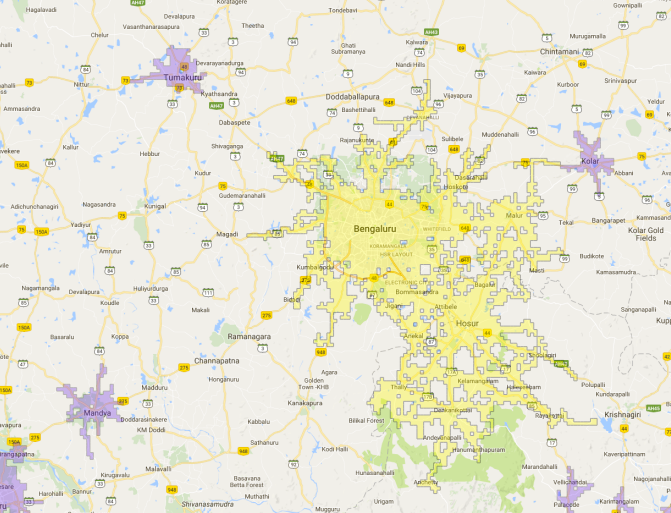
\includegraphics[width=0.8\textwidth]{Bangalore}
  \caption{Geographic Definition of Bangalore}
   \label{fig:Bangalore}
\end{centering}
\end{figure}

\newpage

\begin{figure}[h!]
\begin{centering}
  \includegraphics[width=0.85\textwidth]{countrymoves}
  \caption{Country moves by year}
   \label{fig:countrymoves}
\end{centering}
\end{figure}

\begin{figure}[h!]
\begin{centering}
  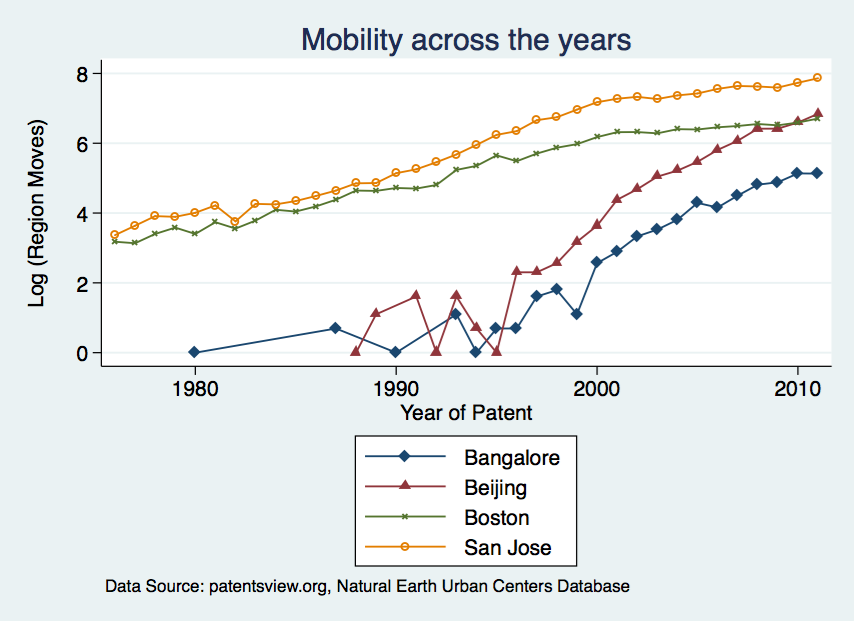
\includegraphics[width=0.85\textwidth]{regionmoves}
  \caption{Region moves by year}
   \label{fig:regionmoves}
\end{centering}
\end{figure}

\newpage
\begin{figure}[h!]
\begin{centering}
  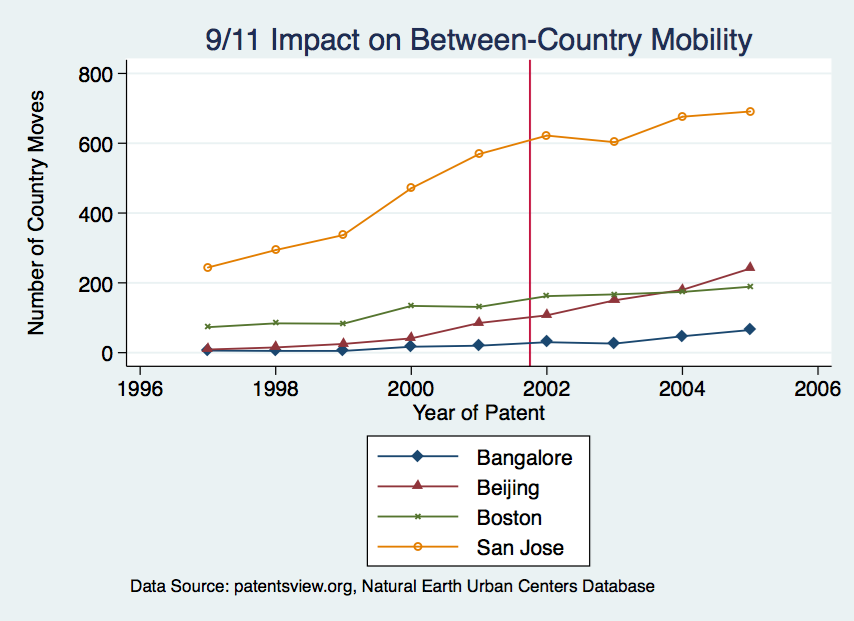
\includegraphics[width=0.85\textwidth]{countrymoves911}
  \caption{9/11 impact on country moves by year}
   \label{fig:countrymoves911}
\end{centering}
\end{figure}

\begin{figure}[h!]
\begin{centering}
  \includegraphics[width=0.85\textwidth]{regionmoves911}
  \caption{9/11 impact on region moves by year}
   \label{fig:regionmoves911}
\end{centering}
\end{figure}

\newpage
\begin{table}[htbp]\centering \caption{Summary statistics \label{sumstat}}
\begin{tabular}{l c c  c}\hline\hline
\multicolumn{1}{c}{\textbf{Variable}} & \textbf{Mean}
 & \textbf{Std. Dev.} & \textbf{N}\\ \hline
moved region & 0.08 & 0.271  & 8537410\\
moved country & 0.029 & 0.166  & 8537410\\
log(complexity) & -1.004 & 2.383  & 7957162\\
inventor pool & 8.542 & 46.674  & 8537410\\
team pool proxy& 27.901 & 112.154  & 6875208\\
\hline
\end{tabular}
\end{table}


\newpage
\begin{table}[htbp]\centering \caption{Most complex technology subclasses in 2010 \label{mostcomplex}}
\begin{tabular}{l c c  c}\hline\hline
\multicolumn{1}{c}{\textbf{id}} & \textbf{Avg Complexity} & \textbf{Technology} \\ \hline
32	&6.691109	&Surgery \& Med Inst.\\
25	&6.583521	&Electronic business methods and software\\
24	&6.361433	&Information Storage\\
22	&5.941292	&Computer Hardware \& Software\\
21	&5.627072	&Communications\\
\hline
\end{tabular}
\end{table}

\begin{table}[htbp]\centering \caption{Least complex technology subclasses in 2010 \label{leastcomplex}}
\begin{tabular}{l c c  c}\hline\hline
\multicolumn{1}{c}{\textbf{id}} & \textbf{Avg Complexity} & \textbf{Technology} \\ \hline
11	&2.533947	&Agriculture,Food,Textiles\\
33	&3.468262	&Genetics\\
66	&3.488879	&Heating\\
52	&3.518574	&Metal Working\\
63	&3.661588	&Apparel \& Textile\\
53	&3.667615	&Motors \& Engines + Parts\\
55	&3.712974	&Transportation\\
\hline
\end{tabular}
\end{table}

\newpage
{
\def\sym#1{\ifmmode^{#1}\else\(^{#1}\)\fi}
\begin{longtable}{l*{3}{c}}
\caption{Preliminary Regression of Mobility of Inventors on Complexity of Inventions \label{model1a1b1c}}\\
\hline\hline\endfirsthead\hline\endhead\hline\endfoot\endlastfoot
                &\multicolumn{1}{c}{(1)}&\multicolumn{1}{c}{(2)}&\multicolumn{1}{c}{(3)}\\
                &\multicolumn{1}{c}{log(complexity)}&\multicolumn{1}{c}{log(complexity)}&\multicolumn{1}{c}{log(complexity)}\\
\hline
moved region    &    0.389\sym{***}&    0.383\sym{***}&    0.957\sym{***}\\
                &  (0.000)         &  (0.000)         &  (0.000)         \\
moved country   &    0.751\sym{***}&    0.736\sym{***}&    1.610\sym{***}\\
                &  (0.000)         &  (0.000)         &  (0.000)         \\
IPR index       &                  &  -0.0371\sym{***}&  -0.0229\sym{***}\\
                &                  &  (0.000)         &  (0.000)         \\
moved region * IPR index&                  &                  &  -0.0601\sym{***}\\
                &                  &                  &  (0.000)         \\
moved country * IPR index&                  &                  &  -0.0964\sym{***}\\
                &                  &                  &  (0.000)         \\
\hline
Observations    &  7957162         &  7918297         &  7918297         \\
$R^2$              &  0.00676         &  0.00721         &  0.00757         \\
Clustered SE              &       No         &       No         &       No         \\
Year Dummies            &       No         &       No         &       No         \\
Sample          &  All Obs         &  All Obs         &  All Obs         \\
\hline\hline
\multicolumn{4}{l}{\footnotesize \textit{p}-values in parentheses}\\
\multicolumn{4}{l}{\footnotesize None of the models include fixed effects, or technology subcategory controls}\\
\multicolumn{4}{l}{\footnotesize \sym{*} \(p<0.05\), \sym{**} \(p<0.01\), \sym{***} \(p<0.001\)}\\
\end{longtable}
}

\newpage
{
\def\sym#1{\ifmmode^{#1}\else\(^{#1}\)\fi}
\begin{longtable}{l*{3}{c}}
\caption{IPR Strength and Mobility of Inventors on Complexity of Inventions \label{model2a2b2c}}\\
\hline\hline\endfirsthead\hline\endhead\hline\endfoot\endlastfoot
                &\multicolumn{1}{c}{(1)}&\multicolumn{1}{c}{(2)}&\multicolumn{1}{c}{(3)}\\
                &\multicolumn{1}{c}{log(complexity)}&\multicolumn{1}{c}{log(complexity)}&\multicolumn{1}{c}{log(complexity)}\\
\hline
moved region    &    0.847\sym{***}&  -0.0635         &    0.270\sym{***}\\
                &  (0.000)         &  (0.559)         &  (0.000)         \\
moved country   &    1.824\sym{***}&    2.385\sym{***}&    1.255\sym{***}\\
                &  (0.000)         &  (0.000)         &  (0.000)         \\
IPR index       &  -0.0257\sym{***}&   0.0773\sym{***}&                  \\
                &  (0.000)         &  (0.000)         &                  \\
moved region * IPR index&  -0.0530\sym{***}&   0.0322\sym{**} &                  \\
                &  (0.000)         &  (0.003)         &                  \\
moved country * IPR index&   -0.110\sym{***}&   -0.189\sym{***}&                  \\
                &  (0.000)         &  (0.000)         &                  \\
strong IPR      &                  &                  &    0.473\sym{***}\\
                &                  &                  &  (0.000)         \\
moved region * strong IPR&                  &                  &  -0.0130         \\
                &                  &                  &  (0.744)         \\
moved country * strong IPR&                  &                  &   -0.833\sym{***}\\
                &                  &                  &  (0.000)         \\
\hline
Observations    &  5280190         &  5280190         &  5280190         \\
$R^2$              &    0.009         &    0.145         &    0.146         \\
Clusters         &  579,806         &  579,806         &  579,806         \\
Clustered SE       &Region Assignee         &Region Assignee         &Region Assignee         \\
Year Dummies            &       No         &      Yes         &      Yes         \\
Sample          &  All Obs         &  All Obs         &  All Obs         \\
\hline\hline
\multicolumn{4}{l}{\footnotesize \textit{p}-values in parentheses}\\
\multicolumn{4}{l}{\footnotesize None of the models include fixed effects, or technology subcategory controls}\\
\multicolumn{4}{l}{\footnotesize \sym{*} \(p<0.05\), \sym{**} \(p<0.01\), \sym{***} \(p<0.001\)}\\
\end{longtable}
}

\newpage
\begin{landscape}
{
\def\sym#1{\ifmmode^{#1}\else\(^{#1}\)\fi}
\begin{longtable}{l*{4}{c}}
\caption{IPR Strength and Mobility of Inventors on Varying Measures of Complexity \label{model3a3b3c3d}}\\
\hline\hline\endfirsthead\hline\endhead\hline\endfoot\endlastfoot
                &\multicolumn{1}{c}{(1)}&\multicolumn{1}{c}{(2)}&\multicolumn{1}{c}{(3)}&\multicolumn{1}{c}{(4)}\\
                &\multicolumn{1}{c}{log(complexity) 2x}&\multicolumn{1}{c}{log(complexity) 3x}&\multicolumn{1}{c}{log(complexity) 4x}&\multicolumn{1}{c}{log(complexity) 5x}\\
\hline
moved region    &    0.270\sym{***}&    0.269         &    0.381         &    0.450         \\
                &  (0.000)         &  (0.072)         &  (0.068)         &  (0.102)         \\
moved country   &    1.255\sym{***}&    2.219\sym{***}&    2.847\sym{***}&    3.490\sym{***}\\
                &  (0.000)         &  (0.000)         &  (0.000)         &  (0.000)         \\
strong IPR      &    0.473\sym{***}&    2.089\sym{***}&    2.823\sym{***}&    3.540\sym{***}\\
                &  (0.000)         &  (0.000)         &  (0.000)         &  (0.000)         \\
moved region * strong IPR&  -0.0130         &  -0.0914         &   -0.122         &   -0.106         \\
                &  (0.744)         &  (0.562)         &  (0.579)         &  (0.715)         \\
moved country * strong IPR&   -0.833\sym{***}&   -2.086\sym{***}&   -2.752\sym{***}&   -3.465\sym{***}\\
                &  (0.000)         &  (0.000)         &  (0.000)         &  (0.000)         \\
\hline
Observations    &  5280190         &   537491         &   460578         &   391121         \\
$R^2$              &    0.146         &    0.026         &    0.026         &    0.026         \\
Clusters         &  579,806         &   91,564         &   80,985         &   71,085         \\
Clustered SE       &Region Assignee         &Region Assignee         &Region Assignee         &Region Assignee         \\
Year Dummies            &      Yes         &      Yes         &      Yes         &      Yes         \\
Sample          &  All Obs         &  All Obs         &  All Obs         &  All Obs         \\
\hline\hline
\multicolumn{5}{l}{\footnotesize \textit{p}-values in parentheses}\\
\multicolumn{5}{l}{\footnotesize None of the models include fixed effects, or technology subcategory controls}\\
\multicolumn{5}{l}{\footnotesize \sym{*} \(p<0.05\), \sym{**} \(p<0.01\), \sym{***} \(p<0.001\)}\\
\end{longtable}
}

\end{landscape}
\newpage
{
\def\sym#1{\ifmmode^{#1}\else\(^{#1}\)\fi}
\begin{longtable}{l*{3}{c}}
\caption{Technology Complexity and Mobility of Inventors on Invention Complexity \label{model4a4b4c}}\\
\hline\hline\endfirsthead\hline\endhead\hline\endfoot\endlastfoot
                &\multicolumn{1}{c}{(1)}&\multicolumn{1}{c}{(2)}&\multicolumn{1}{c}{(3)}\\
                &\multicolumn{1}{c}{log(complexity)}&\multicolumn{1}{c}{log(complexity)}&\multicolumn{1}{c}{log(complexity)}\\
\hline
moved region    &    0.172\sym{***}&    0.183\sym{***}&    0.210         \\
                &  (0.000)         &  (0.000)         &  (0.055)         \\
moved country   &    1.213\sym{***}&    0.305\sym{***}&   0.0599         \\
                &  (0.000)         &  (0.000)         &  (0.700)         \\
strong IPR      &    0.408\sym{***}&                  &                  \\
                &  (0.000)         &                  &                  \\
moved region * strong IPR&   0.0192         &                  &                  \\
                &  (0.590)         &                  &                  \\
moved country * strong IPR&   -0.813\sym{***}&                  &                  \\
                &  (0.000)         &                  &                  \\
moved region * tech complexity&    0.149\sym{***}&    0.250\sym{***}&   0.0448         \\
                &  (0.000)         &  (0.000)         &  (0.734)         \\
moved country * tech complexity&  0.00195         &   -0.123\sym{***}&    0.566\sym{**} \\
                &  (0.927)         &  (0.000)         &  (0.002)         \\
\hline
Observations    &  5245466         &  2599718         &    32095         \\
$R^2$              &    0.169         &    0.251         &    0.124         \\
Clusters         &  575,441         &  323,620         &    4,647         \\
Clustered SE       &Region Assignee         &Region Assignee         &Region Assignee         \\
Year Dummies            &      Yes         &      Yes         &      Yes         \\
Technology Controls            &      Yes         &      Yes         &      Yes         \\
Sample          &  All Obs         &US inventions         &Indian inventions         \\
\hline\hline
\multicolumn{4}{l}{\footnotesize \textit{p}-values in parentheses}\\
\multicolumn{4}{l}{\footnotesize None of the models include fixed effects}\\
\multicolumn{4}{l}{\footnotesize \sym{*} \(p<0.05\), \sym{**} \(p<0.01\), \sym{***} \(p<0.001\)}\\
\end{longtable}
}

\newpage
{
\def\sym#1{\ifmmode^{#1}\else\(^{#1}\)\fi}
\begin{longtable}{l*{1}{c}}
\caption{Extent of Regional Mobility of Inventors on Invention Complexity \label{model5a}}\\
\hline\hline\endfirsthead\hline\endhead\hline\endfoot\endlastfoot
                &\multicolumn{1}{c}{(1)}\\
                &\multicolumn{1}{c}{log(complexity)}\\
\hline
moved region    &  -0.0334         \\
                &  (0.287)         \\
moved country   &    1.089\sym{***}\\
                &  (0.000)         \\
strong IPR      &    0.407\sym{***}\\
                &  (0.000)         \\
moved region * strong IPR&   0.0503         \\
                &  (0.103)         \\
moved country * strong IPR&   -0.727\sym{***}\\
                &  (0.000)         \\
moved region * tech complexity&    0.148\sym{***}\\
                &  (0.000)         \\
moved country * tech complexity&  -0.0181         \\
                &  (0.389)         \\
region moves = 1&  -0.0236\sym{***}\\
                &  (0.000)         \\
region moves = 2&   0.0167         \\
                &  (0.058)         \\
3 <= region moves <= 5&   0.0517\sym{***}\\
                &  (0.000)         \\
6 <= region moves <= 8&    0.120\sym{***}\\
                &  (0.000)         \\
region moves >= 9&    0.488\sym{***}\\
                &  (0.000)         \\
\hline
Observations    &  5245466         \\
$R^2$              &    0.170         \\
Clusters         &  575,441         \\
Clustered SE       &Region Assignee         \\
Year Dummies            &      Yes         \\
Technology Controls            &      Yes         \\
Sample          &  All Obs         \\
\hline\hline
\multicolumn{2}{l}{\footnotesize \textit{p}-values in parentheses}\\
\multicolumn{2}{l}{\footnotesize None of the models include fixed effects}\\
\multicolumn{2}{l}{\footnotesize \sym{*} \(p<0.05\), \sym{**} \(p<0.01\), \sym{***} \(p<0.001\)}\\
\end{longtable}
}

\newpage
{
\def\sym#1{\ifmmode^{#1}\else\(^{#1}\)\fi}
\begin{longtable}{l*{1}{c}}
\caption{Extent of Country Mobility of Inventors on Invention Complexity \label{model5b}}\\
\hline\hline\endfirsthead\hline\endhead\hline\endfoot\endlastfoot
                &\multicolumn{1}{c}{(1)}\\
                &\multicolumn{1}{c}{log(complexity)}\\
\hline
moved region    &   0.0584         \\
                &  (0.073)         \\
moved country   &    0.864\sym{***}\\
                &  (0.000)         \\
strong IPR      &    0.409\sym{***}\\
                &  (0.000)         \\
moved region * strong IPR&   0.0843\sym{*}  \\
                &  (0.012)         \\
moved country * strong IPR&   -0.744\sym{***}\\
                &  (0.000)         \\
moved region * tech complexity&    0.147\sym{***}\\
                &  (0.000)         \\
moved country * tech complexity&  -0.0351         \\
                &  (0.089)         \\
country moves = 1&  -0.0155         \\
                &  (0.156)         \\
country moves = 2&   0.0522\sym{***}\\
                &  (0.000)         \\
country moves = 3&   0.0673\sym{***}\\
                &  (0.000)         \\
country moves = 4&    0.118\sym{***}\\
                &  (0.000)         \\
country moves >= 5&    0.652\sym{***}\\
                &  (0.000)         \\
\hline
Observations    &  5245466         \\
$R^2$              &    0.170         \\
Clusters         &  575,441         \\
Clustered SE       &Region Assignee         \\
Year Dummies            &      Yes         \\
Technology Controls            &      Yes         \\
Sample          &  All Obs         \\
\hline\hline
\multicolumn{2}{l}{\footnotesize \textit{p}-values in parentheses}\\
\multicolumn{2}{l}{\footnotesize None of the models include fixed effects}\\
\multicolumn{2}{l}{\footnotesize \sym{*} \(p<0.05\), \sym{**} \(p<0.01\), \sym{***} \(p<0.001\)}\\
\end{longtable}
}

\newpage
{
\def\sym#1{\ifmmode^{#1}\else\(^{#1}\)\fi}
\begin{longtable}{l*{2}{c}}
\caption{Inventor - Technology Class Controls in Mobility of Inventors on Invention Complexity \label{model6a6b6c}}\\
\hline\hline\endfirsthead\hline\endhead\hline\endfoot\endlastfoot
                &\multicolumn{1}{c}{(1)}&\multicolumn{1}{c}{(2)}\\
                &\multicolumn{1}{c}{log(complexity)}&\multicolumn{1}{c}{log(complexity)}\\
\hline
moved region    &    0.172\sym{***}&    0.135\sym{***}\\
                &  (0.000)         &  (0.000)         \\
moved country   &    1.213\sym{***}&    1.167\sym{***}\\
                &  (0.000)         &  (0.000)         \\
strong IPR      &    0.408\sym{***}&    0.382\sym{***}\\
                &  (0.000)         &  (0.000)         \\
moved region * strong IPR&   0.0192         &   0.0150         \\
                &  (0.590)         &  (0.669)         \\
moved country * strong IPR&   -0.813\sym{***}&   -0.773\sym{***}\\
                &  (0.000)         &  (0.000)         \\
moved region * tech complexity&    0.149\sym{***}&    0.149\sym{***}\\
                &  (0.000)         &  (0.000)         \\
moved country * tech complexity&  0.00195         & 0.000912         \\
                &  (0.927)         &  (0.966)         \\
inventor-tech class&                  &-5.72e-08\sym{***}\\
                &                  &  (0.000)         \\
\hline
Observations    &  5245466         &  5245466         \\
r2              &    0.169         &    0.169         \\
N\_clust         &  575,441         &  575,441         \\
Clustered       &Region Assignee         &Region Assignee         \\
Year            &      Yes         &      Yes         \\
Tech            &      Yes         &      Yes         \\
InventorClass   &       No         &      Yes         \\
Sample          &  All Obs         &  All Obs         \\
\hline\hline
\multicolumn{3}{l}{\footnotesize \textit{p}-values in parentheses}\\
\multicolumn{3}{l}{\footnotesize Unable to add inventor-technology class dummies since there are 4,617,880 unique inventor-technology class tuples}\\
\multicolumn{3}{l}{\footnotesize \sym{*} \(p<0.05\), \sym{**} \(p<0.01\), \sym{***} \(p<0.001\)}\\
\end{longtable}
}

\newpage
{
\def\sym#1{\ifmmode^{#1}\else\(^{#1}\)\fi}
\begin{longtable}{l*{3}{c}}
\caption{Using 9/11 Shock to Estimate the effect of Mobility of Inventors on Invention Complexity \label{model7a7b7c}}\\
\hline\hline\endfirsthead\hline\endhead\hline\endfoot\endlastfoot
                &\multicolumn{1}{c}{(1)}&\multicolumn{1}{c}{(2)}&\multicolumn{1}{c}{(3)}\\
                &\multicolumn{1}{c}{log(complexity)}&\multicolumn{1}{c}{log(complexity)}&\multicolumn{1}{c}{log(complexity)}\\
\hline
moved region    &    0.227\sym{***}&   0.0227         &    0.314\sym{***}\\
                &  (0.000)         &  (0.165)         &  (0.000)         \\
moved country   &    0.151\sym{***}&    0.227\sym{***}&   0.0604         \\
                &  (0.000)         &  (0.000)         &  (0.057)         \\
strong IPR      &   -0.254\sym{***}&                  &   -0.297\sym{***}\\
                &  (0.000)         &                  &  (0.000)         \\
moved region * strong IPR&  -0.0541\sym{**} &                  &  -0.0808\sym{***}\\
                &  (0.006)         &                  &  (0.000)         \\
moved country * strong IPR&  -0.0544         &                  &  -0.0774\sym{*}  \\
                &  (0.071)         &                  &  (0.013)         \\
moved region * tech complexity&-0.000520         &    0.100\sym{***}&  -0.0117         \\
                &  (0.971)         &  (0.000)         &  (0.566)         \\
moved country * tech complexity&   0.0219         &  -0.0444         &   0.0392         \\
                &  (0.242)         &  (0.141)         &  (0.092)         \\
inventor-tech class& 1.78e-08\sym{**} & 3.78e-08\sym{***}&-9.05e-09         \\
                &  (0.001)         &  (0.000)         &  (0.273)         \\
9/11 Shock      &   -0.121\sym{***}&   -0.119\sym{***}&   -0.130\sym{***}\\
                &  (0.000)         &  (0.000)         &  (0.000)         \\
moved region * 9/11&   0.0423\sym{***}&    0.146\sym{***}&  -0.0140         \\
                &  (0.000)         &  (0.000)         &  (0.368)         \\
moved country * 9/11&    0.127\sym{***}&   0.0453         &    0.203\sym{***}\\
                &  (0.000)         &  (0.111)         &  (0.000)         \\
\hline
Observations    &  1578946         &   796535         &   782411         \\
r2              &    0.065         &    0.068         &    0.072         \\
N\_clust         &  223,041         &  124,376         &   98,799         \\
Sample          &  All Obs         &US Inventions         &Non-US Inventions         \\
\hline\hline
\multicolumn{4}{l}{\footnotesize \textit{p}-values in parentheses}\\
\multicolumn{4}{l}{\footnotesize Standard Errors are clustered at the region-assignee level}\\
\multicolumn{4}{l}{\footnotesize All models include year dummies and NBER technology subcategory dummies}\\
\multicolumn{4}{l}{\footnotesize Control for inventor-technology subcategory included}\\
\multicolumn{4}{l}{\footnotesize \sym{*} \(p<0.05\), \sym{**} \(p<0.01\), \sym{***} \(p<0.001\)}\\
\end{longtable}
}

\newpage
{
\def\sym#1{\ifmmode^{#1}\else\(^{#1}\)\fi}
\begin{longtable}{l*{3}{c}}
\caption{Instrumenting with 9/11 Shock to Estimate the effect of Regional Mobility of Inventors on Invention Complexity \label{model8a8b8c}}\\
\hline\hline\endfirsthead\hline\endhead\hline\endfoot\endlastfoot
                &\multicolumn{1}{c}{(1)}&\multicolumn{1}{c}{(2)}&\multicolumn{1}{c}{(3)}\\
                &\multicolumn{1}{c}{log(complexity)}&\multicolumn{1}{c}{log(complexity)}&\multicolumn{1}{c}{log(complexity)}\\
\hline
moved region    &   -23.69\sym{***}&   -6.135\sym{***}&   -16.05\sym{***}\\
                &  (0.000)         &  (0.001)         &  (0.001)         \\
strong IPR      &   -4.212\sym{***}&                  &   -2.777\sym{***}\\
                &  (0.000)         &                  &  (0.000)         \\
moved region * strong IPR&    20.81\sym{***}&                  &    13.32\sym{***}\\
                &  (0.000)         &                  &  (0.001)         \\
moved country * strong IPR&   -2.743\sym{***}&    4.387\sym{***}&   -2.281\sym{**} \\
                &  (0.000)         &  (0.000)         &  (0.001)         \\
moved region * tech complexity&    5.355\sym{***}&    6.278\sym{***}&    5.778\sym{**} \\
                &  (0.000)         &  (0.000)         &  (0.001)         \\
moved country * tech complexity&    4.375\sym{***}&   -4.209\sym{***}&    3.530\sym{***}\\
                &  (0.000)         &  (0.000)         &  (0.001)         \\
inventor-tech class&-0.000000307\sym{***}&-8.79e-08\sym{*}  &-0.000000378\sym{***}\\
                &  (0.000)         &  (0.015)         &  (0.001)         \\
\hline
Observations    &  1578946         &   796535         &   782411         \\
$R^2$              &        .         &        .         &        .         \\
Clusters         &  223,041         &  124,376         &   98,799         \\
Sample          &  All Obs         &US Inventions         &Non-US Inventions         \\
\hline\hline
\multicolumn{4}{l}{\footnotesize \textit{p}-values in parentheses}\\
\multicolumn{4}{l}{\footnotesize Standard Errors are clustered at the region-assignee level}\\
\multicolumn{4}{l}{\footnotesize All models include year dummies and NBER technology subcategory dummies}\\
\multicolumn{4}{l}{\footnotesize Control for inventor-technology subcategory included}\\
\multicolumn{4}{l}{\footnotesize \sym{*} \(p<0.05\), \sym{**} \(p<0.01\), \sym{***} \(p<0.001\)}\\
\end{longtable}
}

\newpage
{
\def\sym#1{\ifmmode^{#1}\else\(^{#1}\)\fi}
\begin{longtable}{l*{3}{c}}
\caption{Instrumenting with 9/11 Shock to Estimate the effect of Regional Mobility of Inventors on Invention Complexity \label{model9a9b9c}}\\
\hline\hline\endfirsthead\hline\endhead\hline\endfoot\endlastfoot
                &\multicolumn{1}{c}{(1)}&\multicolumn{1}{c}{(2)}&\multicolumn{1}{c}{(3)}\\
                &\multicolumn{1}{c}{log(complexity)}&\multicolumn{1}{c}{log(complexity)}&\multicolumn{1}{c}{log(complexity)}\\
\hline
moved region    &   -23.69\sym{***}&   -6.135\sym{***}&   -16.05\sym{***}\\
                &  (0.000)         &  (0.001)         &  (0.001)         \\
strong IPR      &   -4.212\sym{***}&                  &   -2.777\sym{***}\\
                &  (0.000)         &                  &  (0.000)         \\
moved region * strong IPR&    20.81\sym{***}&                  &    13.32\sym{***}\\
                &  (0.000)         &                  &  (0.001)         \\
moved country * strong IPR&   -2.743\sym{***}&    4.387\sym{***}&   -2.281\sym{**} \\
                &  (0.000)         &  (0.000)         &  (0.001)         \\
moved region * tech complexity&    5.355\sym{***}&    6.278\sym{***}&    5.778\sym{**} \\
                &  (0.000)         &  (0.000)         &  (0.001)         \\
moved country * tech complexity&    4.375\sym{***}&   -4.209\sym{***}&    3.530\sym{***}\\
                &  (0.000)         &  (0.000)         &  (0.001)         \\
\hline
Observations    &  1578946         &   796535         &   782411         \\
$R^2$              &        .         &        .         &        .         \\
Clusters         &  223,041         &  124,376         &   98,799         \\
F              &       26         &       66         &       21         \\
Sample          &  All Obs         &US Inventions         &Non-US Inventions         \\
\hline\hline
\multicolumn{4}{l}{\footnotesize \textit{p}-values in parentheses}\\
\multicolumn{4}{l}{\footnotesize Standard Errors are clustered at the region-assignee level}\\
\multicolumn{4}{l}{\footnotesize All models include year dummies and NBER technology subcategory dummies}\\
\multicolumn{4}{l}{\footnotesize Control for inventor-technology subcategory included}\\
\multicolumn{4}{l}{\footnotesize \sym{*} \(p<0.05\), \sym{**} \(p<0.01\), \sym{***} \(p<0.001\)}\\
\end{longtable}
}


\end{document}
